%Do not change these lines, just uncomment the needed one
%\documentclass[prd,twocolumn,showpacs,groupedaddress,superscriptaddress,amsmath,amssymb]{revtex4-2}
\documentclass[prd,showpacs,groupedaddress,superscriptaddress,amsmath,amssymb]{revtex4-2} % one-column text
%\documentclass[preprint,showpacs,amsmath,amssymb]{revtex4-2}

\usepackage{hhline}
\usepackage{slashed}
\usepackage{graphicx}% Include figure files
\usepackage{graphics}
\usepackage{dcolumn}% Align table columns on decimal point
\usepackage{bm}% bold math
\usepackage{amssymb}
\usepackage{enumerate}
\usepackage{lineno}
\usepackage{multirow}
%\usepackage{footnote}

%\linenumbers


\textwidth19.0cm
\textheight24.0cm
\setlength{\topmargin}{-1.5cm}
\oddsidemargin -1.cm
\evensidemargin 2.cm
\def\u{\tilde{u}}
\def\s{\tilde{s}}
\def\t{\tilde{t}}
\def\P{\mathcal{P}}
\def\u{\tilde{u}}
\def\s{\tilde{s}}
\def\t{\tilde{t}}
\def\k{{\bf k}}
\def\p{{\bf p }}
\def\V{{\bf V}}

\newcommand\ee{e^+e^-}
\newcommand\xdecay{X \rightarrow e^+  e^-}
\newcommand\ainv{A'\to invisible}
\newcommand\inv{ \chi\overline{\chi}}
\newcommand\gp{ A'}
\newcommand\g{\gamma}
\newcommand\ma{m_{A'}}
\newcommand\pair{e^+e^-}
\newcommand\na{{n}_{A'}}
\newcommand\Na{{N}_{A'}}
\newcommand\ea{e^- Z \to e^- Z A';~ A' \to \chi \overline{\chi}}
\newcommand\emu{e^- Z \to e^- Z \g; \g \to \mu^+ \mu^-}
\newcommand\mm{\mu^+ \mu^-}


\begin{document}


%For CERN preprint:
%\begin{center}
%{\Large EUROPEAN ORGANIZATION FOR NUCLEAR RESEARCH}
%\end{center}
%\vskip1.5cm
%\begin{flushright}
%CERN-EP-2019-.....\\
%\today
%\end{flushright}
%end CERN preprint


\title{ \bf Study of sensitivities of the P2O project}


\author{M.~M.~Kirsanov$^{1}$\thanks{{\bf e-mail}: mikhail.m.kirsanov@gmail.com}, A.~Sokolov$^{2}$
\\
 $^1$ Institute for Nuclear Research of the Russian Academy of Sciences, \\117312 Moscow, Russia \\
 $^2$ Institute for High Energy Physics, Protvino, Russia \\
}


%alternative way of writing authors list, with a possibility of e-mail for several authors 
%\author{M. M. Kirsanov}
%\thanks{Corresponding author}
%\email[\textbf{e-mail}: ]{mikhail.kirsanov@cern.ch}
%\affiliation{Institute for Nuclear Research, 117312 Moscow, Russia}
%\author{N.~V.~Krasnikov}
%\email[\textbf{e-mail}: ]{nikolai.krasnikov@cern.ch}
%\affiliation{Institute for Nuclear Research, 117312 Moscow, Russia}
%\affiliation{Joint Institute for Nuclear Research, 141980 Dubna, Russia}


%For the collaboration papers:
%\input ../AUTHORS/author_list.tex


\date{\today}% It is always \today, today,
             %  but any date may be explicitly specified
%\date{June 17, 2009}% It is always \today, today,
             %  but any date may be explicitly specified



\begin{abstract}
The sensitivities of the project to some oscillation parameters as a function of power and systematic errors are studied.
\end{abstract}


\maketitle
\newpage


\section{Introduction}


 P2O is the project of neutrino beam from IHEP Protvino to ORCA \cite{Akindinov:2019flp}


\section{Technical notes on the repository}


 The files for this project, including Papers and Notes, are kept in https://github.com/kirsanov-protvino/P2O . In order to work
on them one should create account on github. Next step is to create an SSH key. Add this key to your account on the page https://github.com/settings/keys.
After that you will be able to clone the repository using the command git clone git@github.com:kirsanov-protvino/P2O.git and push your changes in it.
The command above is shown when you click the green button "Code" on the repository page and switch to SSH instead of HTTPS.
To check that your repositiry clone is "pushable" type inside it "git remote -v".


\section{Technical notes on the Globes program running}


 In order to check that the statistics corresponds to the Proposal, the following call was used: \\
glbGetChannelRatePtr(0, ichannel, GLB\_PRE).
It returns the numbers of events in energy bins, to be summed over the them. It is to be called AFTER the calculation of sensitivities,
otherwise some variables are not initialized. It is found that with the normalization factor 40 in the glb file the total number of
events corresponds to the one in Figure 7 of the Proposal \cite{Akindinov:2019flp} (20000 $\nu_{\mu}CC$ events by eye from the figure).


\section{Study of the experiment resolution}


 The resolution of $\delta$ measurement for the true value $\delta = \pi/2$ is shown in Fig. \ref{fig:del_delres_eres}.


\begin{figure*}[h]
\begin{center}
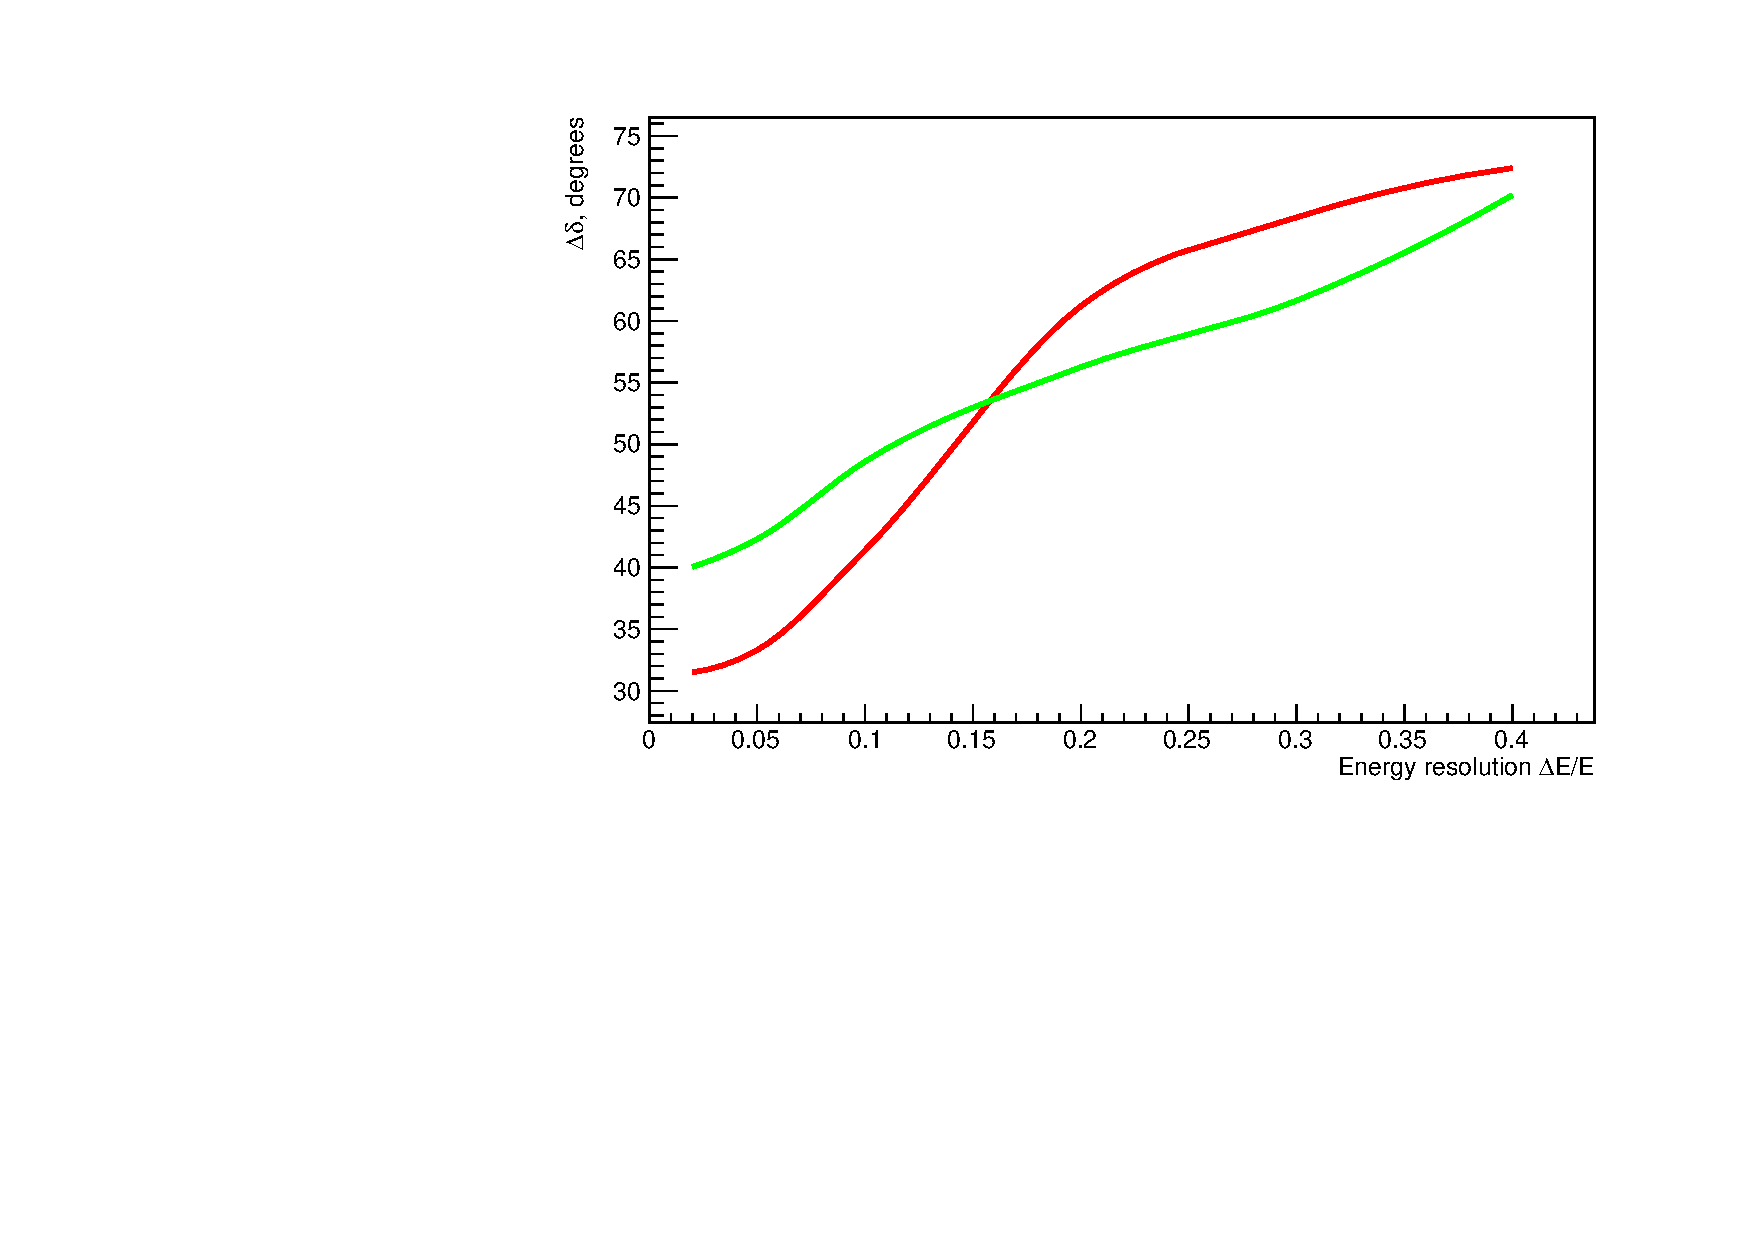
\includegraphics[width=0.75\textwidth]{del_delres_eres.pdf}
\caption {Resolution of the $\delta$ measurement as a function of energy resolution
\label{fig:del_delres_eres}}
\end{center}
\end{figure*}




\clearpage
\bibliographystyle{apsrev4-2}
\bibliography{../Bibliography/bibliographyP2O}


\end{document}
